\section{Operational MILP and scenario-to-model mapping}
\label{app:milp}
This appendix describes the implemented formulation, not a generic unit
commitment model. All parameters below are fixed by scenario $s$.
The code-level specification is \texttt{src/milp/model.py}, with the
time-unit correction and independent validator in
\texttt{src/operational\_exit/physics.py}. The reproducibility archive
records their exact hashes and the scenario loader and profile generator.

\paragraph{Indices, variables and aggregation.}
Let $z\in\mathcal Z$, $t=1,\ldots,T$, $\ell\in\mathcal L$ and
$k\in\mathcal K_{\rm DR}$ index zones, time, transport lines and response
cost blocks. Powers and flows are in MW; stored and deferred energy are in
MWh; $\Delta t$ is in hours. Continuous nonnegative variables are thermal,
nuclear, solar, wind and hydro generation $p^{\rm th},p^{\rm nu},p^{\rm sol},
p^{\rm wind},h$; renewable and hydro spill; battery and pumped charge,
discharge and energy; deferred power $d$, recovered power $r$, backlog $q$;
ENS $e$; overgeneration spill $o$; and system imports $m^+$ and exports $m^-$.
Transport flows $f_{\ell t}$ may be positive or negative. Binary variables
are thermal on/off $u_{zt}$ and start-up $v_{zt}$, deferral activation $a_{zt}$,
battery/pumped charge modes $c^B_{zt},c^P_{zt}$ and import mode $i_t$.
There is one thermal commitment per zone and time, not one per installed
thermal unit. Nuclear output is continuous and subject to minimum output;
there is no nuclear commitment binary. Shutdown is the expression
$w_{zt}=u_{z,t-1}-u_{zt}+v_{zt}$, not an additional decision variable.

\paragraph{Generator metadata are not always active physical controls.}
The historical JSON files omit the optional unit-capacity override block.
Installed battery energy therefore equals installed battery power times the
loader's default four hours. The sampled field
\path{battery_e_to_p_hours} enters generator flexibility summaries and B8,
but does not change that installed duration in this cohort. Likewise,
\path{dr_duration_hours} does not impose a maximum deferral duration in the
implemented lossless-backlog constraints, and the nominal hydro head-efficiency
field is not an extra multiplier in the nodal balance. These legacy fields
must not be described as independently varied physical constraints. Their
predictive associations can reflect sampling correlations. New physical
duration experiments must explicitly change realized power/energy arrays,
as the prepared decoupling batch does.

\paragraph{Objective.}
The validated objective, including trade credits and unserved-energy cost, is
\begin{align}
 \min\ C={}&\sum_{z,t} c^{\rm start}_zv_{zt}
 +\Delta t\sum_{z,t}\left(c^{\rm th}_zp^{\rm th}_{zt}
 +c^{\rm nu}_zp^{\rm nu}_{zt}+\sum_k c^{\rm DR}_kd_{ztk}
 +V e_{zt}+c^{\rm ren}(s^{\rm sol}_{zt}+s^{\rm wind}_{zt})\right.\nonumber\\
 &\left.\qquad+c^{\rm hydro}s^H_{zt}+c^o o_{zt}
 +c^B_z(p^{B+}_{zt}+p^{B-}_{zt})
 +c^P_z(p^{P+}_{zt}+p^{P-}_{zt})\right)\nonumber\\
 &+\Delta t\sum_t(c^{\rm imp}m^+_t+c^{\rm exp}m^-_t).
\end{align}
Here $c^{\rm exp}$ is negative. The thermal energy cost includes fuel,
the variable operating adder and $0.72$ times the carbon price.
Start-up costs are charged per event, without multiplication by $\Delta t$.
The historical references may consequently have negative total cost.
The metadata nuclear start-up cost does not enter an additional nuclear
commitment term in this implemented MILP.

\paragraph{Thermal and nuclear operation.}
Initial output and on/off state are scenario parameters. For every zone and
time, thermal constraints are
\begin{align}
 \underline P^{\rm th}_zu_{zt}&\le p^{\rm th}_{zt}\le\overline P^{\rm th}_zu_{zt},\\
 v_{zt}&\ge u_{zt}-u_{z,t-1},\quad
 v_{zt}\le u_{zt},\quad v_{zt}\le1-u_{z,t-1},\\
 p^{\rm th}_{zt}-p^{\rm th}_{z,t-1}
 &\le R_zu_{z,t-1}+SU_zv_{zt},\\
 p^{\rm th}_{z,t-1}-p^{\rm th}_{zt}
 &\le R_zu_{zt}+SD_zw_{zt}.
\end{align}
The shared thermal-limit routine determines $SU_z,SD_z$ and initial status;
the inequalities apply also at the first step using those initial values.
No thermal minimum-up/down-duration constraints are imposed. Nuclear output
satisfies $\underline P^{\rm nu}_z\le p^{\rm nu}_{zt}\le\overline P^{\rm nu}_z$
and $|p^{\rm nu}_{zt}-p^{\rm nu}_{z,t-1}|\le0.5\overline P^{\rm nu}_z$ for
$t>1$. Solar and wind each satisfy $p^{j}_{zt}+s^{j}_{zt}=\overline P^j_{zt}$.

\paragraph{Lossless deferred demand.}
Block variables sum to total deferral:
\begin{align}
 d_{zt}&=\sum_kd_{ztk},\quad0\le d_{ztk}\le\overline D_{ztk},\quad
 0.1a_{zt}\le d_{zt}\le\overline D_{zt}a_{zt},\\
 0\le r_{zt}&\le\overline R_{zt}(1-a_{zt}),\quad
 q_{zt}=q_{z,t-1}+\Delta t(d_{zt}-r_{zt}),\\
 \Delta t\,r_{zt}&\le q_{z,t-1},\quad q_{z0}=q_{zT}=0,\quad q_{zt}\ge0,\\
 \sum_t a_{zt}&\le M_z,\qquad |d_{zt}-d_{z,t-1}|\le R^{\rm DR}_z\quad(t>1).
\end{align}
The parameter historically named \texttt{dr\_max\_events} limits active
periods, not activation starts. The legacy minimum-duration field does not
add a minimum-duration constraint. Rebound decay and terminal backlog
tolerance fields do not override the implemented lossless balance and exact
terminal repayment. Unserved energy $e$ is a separate penalized variable;
it is never identified with temporary deferral $d$.

\paragraph{Storage and hydro.}
For $j\in\{B,P\}$ (battery or pumped storage),
\begin{align}
 0\le p^{j+}_{zt}&\le\overline P^j_zc^j_{zt},\quad
 0\le p^{j-}_{zt}\le\overline P^j_z(1-c^j_{zt}),\\
 E^j_{zt}&=\rho^j_zE^j_{z,t-1}
 +\Delta t\left(\eta^{j+}p^{j+}_{zt}-p^{j-}_{zt}/\max(\eta^{j-},10^{-4})\right),\\
 0\le E^j_{zt}&\le\overline E^j_z,\qquad
 \underline E^j_{zT}\le E^j_{zT}\le\overline E^j_{zT}.
\end{align}
Initial levels are fixed. Terminal inequalities are activated in the code
when the associated capacity and bound exceed $10^{-6}$; otherwise the
ordinary nonnegativity/capacity bounds apply. Zero-energy pumped devices
have their level fixed to zero. Reservoir hydro satisfies
\begin{equation}
 H_{zt}=H_{z,t-1}+\Delta t(I_{zt}-h_{zt}-s^H_{zt}),\quad
 0\le H_{zt}\le\overline H_z,\quad0\le h_{zt}\le\overline P^H_z,
\end{equation}
with fixed initial reservoir level; no reservoir terminal target is imposed.
Zero-energy reservoirs are fixed to zero. Run-of-river generation is fixed
scenario input. Hydro release is already represented as electrical power
in the balance; no additional efficiency multiplier is inserted there.

\paragraph{Transport, trade and power balance.}
Let $A_{z\ell}$ be $+1$ at the receiving endpoint and $-1$ at the sending
endpoint, and $z_0$ the import/export anchor zone. Then
\begin{align}
 -\overline F_\ell&\le f_{\ell t}\le\overline F_\ell,\qquad
 0\le m^+_t\le\overline M i_t,\quad0\le m^-_t\le\overline M(1-i_t),\\
 &p^{\rm th}_{zt}+p^{\rm nu}_{zt}+p^{\rm sol}_{zt}+p^{\rm wind}_{zt}
 +h_{zt}+p^{\rm ror}_{zt}+p^{B-}_{zt}+p^{P-}_{zt}
 +\sum_\ell A_{z\ell}f_{\ell t}\nonumber\\
 &\quad+\ind\{z=z_0\}(m^+_t-m^-_t)+d_{zt}+e_{zt}
 =D_{zt}+r_{zt}+p^{B+}_{zt}+p^{P+}_{zt}+o_{zt}.
\end{align}
There are no electrical angles, Kirchhoff loop equations, AC losses or
security contingencies. Binary variables attached to absent thermal,
storage, response or trade capacity are fixed to zero. These structural
fixings are one reason the generator estimate B3 is not a count of actual
free binary variables.

\section{Additional revision protocols and reproducibility}
\label{app:revision_protocol}
The common-direction regression is
\begin{equation}
 \widehat Y^{(p)}_{sb}=a^{(p)}_b+\alpha^{(p)}_b\sum_jw^{(p)}_jz_{sj},
 \quad w_j\ge0,\quad\sum_jw_j=1,\quad\alpha_b\ge0.
\end{equation}
Its objective is the mean squared loss over scenarios and deadlines plus
$\lambda |\mathcal D|^{-1}\sum_b\|\alpha_bw\|_2^2$. This reduces to the
common-vector penalty when all amplitudes are equal. Alternating
nonnegative least squares uses pooled, uniform-active and B1-coordinate
initializations for the full design; other representations use their first
coordinate when B1 is absent. Initialization objectives, convergence and
outer-fold group-weight sums are retained. A shared direction is not
claimed globally optimal merely because the alternating procedure converges.

The conditional models use a fractional Bernoulli quasi-likelihood with
logistic link; binary targets are its special case. Training subsets are
restricted to the stated conditioning event. Single-class subsets use the
observed constant; empty subsets use 0.5 and other subsets with fewer than
ten observations use Laplace-smoothed frequency. A common penalty for the
E/ES factors is selected by their mean inner-fold Brier loss, preserving
probability ordering. For continuous loss,
\begin{equation}
 \widehat{\mathbb E}[Y^{(p)}\mid x,b]
 =1-\widehat P(F\mid x,b)
 +\widehat P(F\mid x,b)\widehat{\mathbb E}[Y^{(p)}\mid F,x,b].
\end{equation}
The linear candidate grid is $\{0,10^{-4},10^{-3},10^{-2},10^{-1},1,10\}$;
constant and original-index fits remain unpenalized. Boosting uses 100
iterations, learning rate 0.05, leaf counts selected from $\{7,15,31\}$,
minimum leaf size 20 and $L_2=1$, with early stopping disabled. Reduced
features are chosen inside each training fold by discarding constants
and then correlations exceeding 0.95 in absolute value, in fixed component
order. The nonsaturating sensitivity replaces only A6 and B8 with
$0.5+\arctan((x-\ell)/(u-\ell)-0.5)/\pi$ using their raw values.

The one-at-a-time target grid varies ENS anchors over 0.005/0.01/0.02,
cost-gap anchors over 0.025/0.05/0.10, and carbon-intensity anchors over
0.36/0.72/1.44. Priority weights are 0.4/0.6/0.8 with equal sharing of the
remainder. The physical emissions factor remains 0.72. A separate
evaluation removes ENS penalties and thermal carbon charges from both
candidate and reference costs; it evaluates the same dispatches and does
not reoptimize them. Binary label counts are checked at 1/5/10\% cost
tolerances. These are sensitivity conventions, not scientifically
estimated thresholds. Imports retain unknown emissions rather than an
assumed zero footprint.

\begin{figure}[htbp]\centering
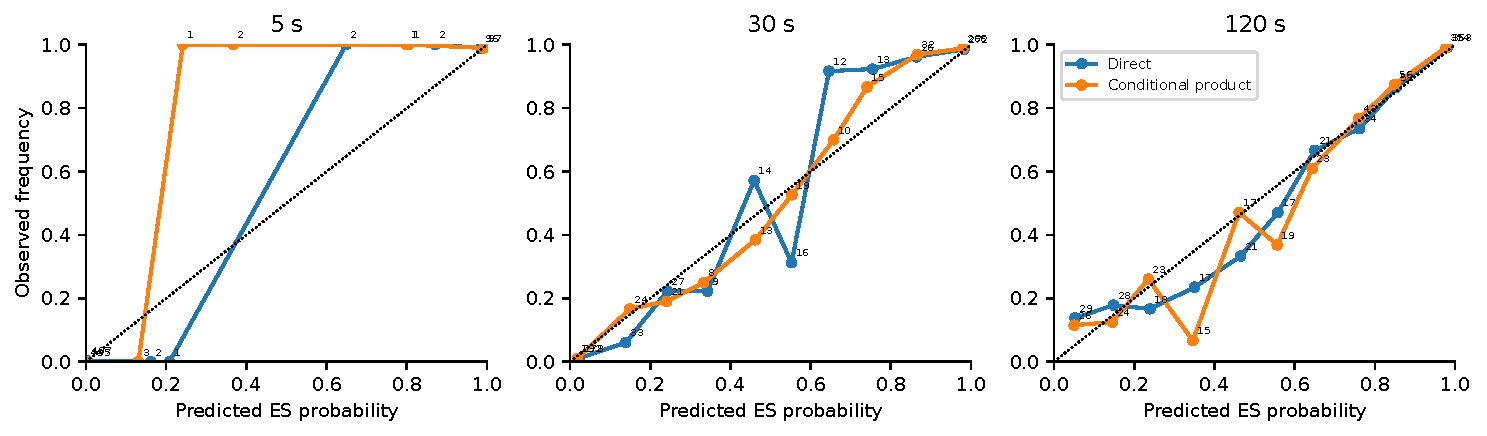
\includegraphics[width=\linewidth]{paper1/results/revision_calibration.pdf}
\caption{ES calibration in the revision models. Labels give observation
counts in fixed probability bins; sparse bins should not be overinterpreted.}
\end{figure}

The unified data contain four Parquet tables (scenarios, runs, references
and analysis) and \path{splits.json} in the isolated revision run.

All raw and normalized
descriptors, identities, families, actual available dimensions, missing
fields, reference certification and process-exit outcomes are retained.
The dictionary specifies formulas, units, input sources, floors, clipping
and fixed normalization bounds for all 22 components. Per-scenario
parameters and family-wise ranges are exported separately; the original
generator configuration and family-building scripts specify the sampling
and selection process. Historical environment versions are HiGHS 1.14.0,
Pyomo 6.10.0 and Python 3.11.9 on Windows, with 16 solver threads. Model
fitting uses the recorded numerical-library versions and one numerical
thread. Historical fold seed is 20261111; revision randomization seed is
20261112. Exact folds and per-execution seeds take precedence over a single
global seed. Historical archives do not identify all stage times or a
complete contemporaneous hardware record; these are not inferred from
total execution time or from the current machine.

The four independent batches currently being executed contain 100 cases each. Temporal
conditions are (12,60), (48,60), (72,60), (24,30), (24,120), in hours and
minutes per step. Topologies vary edges independently of zone count while
remaining connected transport networks. Decoupled conditions vary storage
power and energy factors independently over $[0.5,2]$ and reshape demand
while preserving its total energy. Both generator-proxy and realized-descriptor
predictors were frozen before the first independent attempt. Their ability
to represent the changed inputs is part of the evaluation; historically
constant coordinates still have no learned effect. The later bounded-model
follow-up is stored separately and does not replace this freeze. The strengthened
reference budget is 1,800 solver seconds with a 2,100-second process cap.
No independent performance estimate is reported in this revision. The ongoing
instrumented worker records scenario processing, model construction,
solver transfer, solution search, extraction, validation and delivery,
while the parent supervisor measures complete process exit. Partial stage
logs from interrupted runs cannot turn those runs into successes.
